\documentclass{ximera}

%\usepackage{todonotes}

\newcommand{\todo}{}

\usepackage{tkz-euclide}
\tikzset{>=stealth} %% cool arrow head
\tikzset{shorten <>/.style={ shorten >=#1, shorten <=#1 } } %% allows shorter vectors

\usepackage{tkz-tab}  %% sign charts
\usetikzlibrary{decorations.pathreplacing} 

\usetikzlibrary{backgrounds} %% for boxes around graphs
\usetikzlibrary{shapes,positioning}  %% Clouds and stars
\usetikzlibrary{matrix} %% for matrix
\usepgfplotslibrary{polar} %% for polar plots
\usetkzobj{all}
\usepackage[makeroom]{cancel} %% for strike outs
%\usepackage{mathtools} %% for pretty underbrace % Breaks Ximera
\usepackage{multicol}

\usepackage{polynom}



\usepackage[many]{tcolorbox}  %% for titled boxes
\newtcolorbox{xbox}[1]{%
    tikznode boxed title,
    enhanced,
    arc=0mm,
    interior style={white},
    attach boxed title to top center= {yshift=-\tcboxedtitleheight/2},
    fonttitle=\bfseries,
    colbacktitle=white,coltitle=black,
    boxed title style={size=normal,colframe=white,boxrule=0pt},
    title={#1}}


\usepackage{array}
\setlength{\extrarowheight}{+.1cm}   
\newdimen\digitwidth
\settowidth\digitwidth{9}
\def\divrule#1#2{
\noalign{\moveright#1\digitwidth
\vbox{\hrule width#2\digitwidth}}}





\newcommand{\RR}{\mathbb R}
\newcommand{\R}{\mathbb R}
\newcommand{\N}{\mathbb N}
\newcommand{\Z}{\mathbb Z}

%\renewcommand{\d}{\,d\!}
\renewcommand{\d}{\mathop{}\!d}
\newcommand{\dd}[2][]{\frac{\d #1}{\d #2}}
\newcommand{\pp}[2][]{\frac{\partial #1}{\partial #2}}
\renewcommand{\l}{\ell}
\newcommand{\ddx}{\frac{d}{\d x}}
\newcommand{\ddt}{\frac{d}{\d t}}

\newcommand{\zeroOverZero}{\ensuremath{\boldsymbol{\tfrac{0}{0}}}}
\newcommand{\inftyOverInfty}{\ensuremath{\boldsymbol{\tfrac{\infty}{\infty}}}}
\newcommand{\zeroOverInfty}{\ensuremath{\boldsymbol{\tfrac{0}{\infty}}}}
\newcommand{\zeroTimesInfty}{\ensuremath{\small\boldsymbol{0\cdot \infty}}}
\newcommand{\inftyMinusInfty}{\ensuremath{\small\boldsymbol{\infty - \infty}}}
\newcommand{\oneToInfty}{\ensuremath{\boldsymbol{1^\infty}}}
\newcommand{\zeroToZero}{\ensuremath{\boldsymbol{0^0}}}
\newcommand{\inftyToZero}{\ensuremath{\boldsymbol{\infty^0}}}



\newcommand{\numOverZero}{\ensuremath{\boldsymbol{\tfrac{\#}{0}}}}
\newcommand{\dfn}{\textbf}
%\newcommand{\unit}{\,\mathrm}
\newcommand{\unit}{\mathop{}\!\mathrm}
\newcommand{\eval}[1]{\bigg[ #1 \bigg]}
\newcommand{\seq}[1]{\left( #1 \right)}
\renewcommand{\epsilon}{\varepsilon}
\renewcommand{\iff}{\Leftrightarrow}

\DeclareMathOperator{\arccot}{arccot}
\DeclareMathOperator{\arcsec}{arcsec}
\DeclareMathOperator{\arccsc}{arccsc}
\DeclareMathOperator{\si}{Si}
\DeclareMathOperator{\proj}{proj}
\DeclareMathOperator{\scal}{scal}


\newcommand{\tightoverset}[2]{% for arrow vec
  \mathop{#2}\limits^{\vbox to -.5ex{\kern-0.75ex\hbox{$#1$}\vss}}}
\newcommand{\arrowvec}[1]{\tightoverset{\scriptstyle\rightharpoonup}{#1}}
\renewcommand{\vec}{\mathbf}
\newcommand{\veci}{\vec{i}}
\newcommand{\vecj}{\vec{j}}
\newcommand{\veck}{\vec{k}}
\newcommand{\vecl}{\boldsymbol{\l}}

\newcommand{\dotp}{\bullet}
\newcommand{\cross}{\boldsymbol\times}
\newcommand{\grad}{\boldsymbol\nabla}
\newcommand{\divergence}{\grad\dotp}
\newcommand{\curl}{\grad\cross}
%\DeclareMathOperator{\divergence}{divergence}
%\DeclareMathOperator{\curl}[1]{\grad\cross #1}


\colorlet{textColor}{black} 
\colorlet{background}{white}
\colorlet{penColor}{blue!50!black} % Color of a curve in a plot
\colorlet{penColor2}{red!50!black}% Color of a curve in a plot
\colorlet{penColor3}{red!50!blue} % Color of a curve in a plot
\colorlet{penColor4}{green!50!black} % Color of a curve in a plot
\colorlet{penColor5}{orange!80!black} % Color of a curve in a plot
\colorlet{fill1}{penColor!20} % Color of fill in a plot
\colorlet{fill2}{penColor2!20} % Color of fill in a plot
\colorlet{fillp}{fill1} % Color of positive area
\colorlet{filln}{penColor2!20} % Color of negative area
\colorlet{fill3}{penColor3!20} % Fill
\colorlet{fill4}{penColor4!20} % Fill
\colorlet{fill5}{penColor5!20} % Fill
\colorlet{gridColor}{gray!50} % Color of grid in a plot

\newcommand{\surfaceColor}{violet}
\newcommand{\surfaceColorTwo}{redyellow}
\newcommand{\sliceColor}{greenyellow}




\pgfmathdeclarefunction{gauss}{2}{% gives gaussian
  \pgfmathparse{1/(#2*sqrt(2*pi))*exp(-((x-#1)^2)/(2*#2^2))}%
}


%%%%%%%%%%%%%
%% Vectors
%%%%%%%%%%%%%

%% Simple horiz vectors
\renewcommand{\vector}[1]{\left\langle #1\right\rangle}


%% %% Complex Horiz Vectors with angle brackets
%% \makeatletter
%% \renewcommand{\vector}[2][ , ]{\left\langle%
%%   \def\nextitem{\def\nextitem{#1}}%
%%   \@for \el:=#2\do{\nextitem\el}\right\rangle%
%% }
%% \makeatother

%% %% Vertical Vectors
%% \def\vector#1{\begin{bmatrix}\vecListA#1,,\end{bmatrix}}
%% \def\vecListA#1,{\if,#1,\else #1\cr \expandafter \vecListA \fi}

%%%%%%%%%%%%%
%% End of vectors
%%%%%%%%%%%%%

%\newcommand{\fullwidth}{}
%\newcommand{\normalwidth}{}



%% makes a snazzy t-chart for evaluating functions
%\newenvironment{tchart}{\rowcolors{2}{}{background!90!textColor}\array}{\endarray}

%%This is to help with formatting on future title pages.
\newenvironment{sectionOutcomes}{}{} 



%% Flowchart stuff
%\tikzstyle{startstop} = [rectangle, rounded corners, minimum width=3cm, minimum height=1cm,text centered, draw=black]
%\tikzstyle{question} = [rectangle, minimum width=3cm, minimum height=1cm, text centered, draw=black]
%\tikzstyle{decision} = [trapezium, trapezium left angle=70, trapezium right angle=110, minimum width=3cm, minimum height=1cm, text centered, draw=black]
%\tikzstyle{question} = [rectangle, rounded corners, minimum width=3cm, minimum height=1cm,text centered, draw=black]
%\tikzstyle{process} = [rectangle, minimum width=3cm, minimum height=1cm, text centered, draw=black]
%\tikzstyle{decision} = [trapezium, trapezium left angle=70, trapezium right angle=110, minimum width=3cm, minimum height=1cm, text centered, draw=black]



\\outcome{Derive the derivatives of inverse trigonometric functions.}
\outcome{Understand how the derivative of an inverse function relates to the original derivative.}
\outcome{Take derivatives which involve inverse trigonometric functions.}

\title[Dig-In:]{Derivatives of inverse trigonometric functions}

\begin{document}
\begin{abstract}
  We derive the derivatives of inverse trigonometric functions using implicit
  differentiation.
\end{abstract}
\maketitle

Now we will derive the derivative of arcsine, arctangent, and
arcsecant.

%% Since this is an inverse
%% function, we can find its derivative by using implicit
%% differentiation and the Inverse Function Theorem.


\begin{theorem}[The derivative of arcsine]\index{derivative!of arcsine}
\[
\ddx \arcsin(x) = \frac{1}{\sqrt{1-x^2}}.
\]
\begin{explanation} 
  %% To start, note that the Inverse Function Theorem assures us that this
  %% derivative actually exists.
  Recall
  \[
  \arcsin(x) = \theta
  \]
  means that $\sin(\theta) = x$ and $\answer[given]{\frac{-\pi}{2}}\le
  \theta\le \answer[given]{\frac{\pi}{2}}$.
  Implicitly differentiating with respect $x$ we see
  \begin{align*}
    \sin(\theta) &= x\\
    \ddx \sin(\theta) &= \ddx x &\text{Differentiate both sides.}\\
    \cos(\theta) \cdot \theta' &= 1 &\text{Implicit differentiation.}\\
    \theta' &= \frac{1}{\cos(\theta)} &\text{Solve for $\theta'$.}
  \end{align*}
  While $\theta' = \frac{1}{\cos(\theta)}$, we need our answer written
  in terms of $x$. Since we are assuming that
  \[
  \sin(\theta) = x,
  \]
  consider the following triangle with the unit circle:
  \begin{image}
    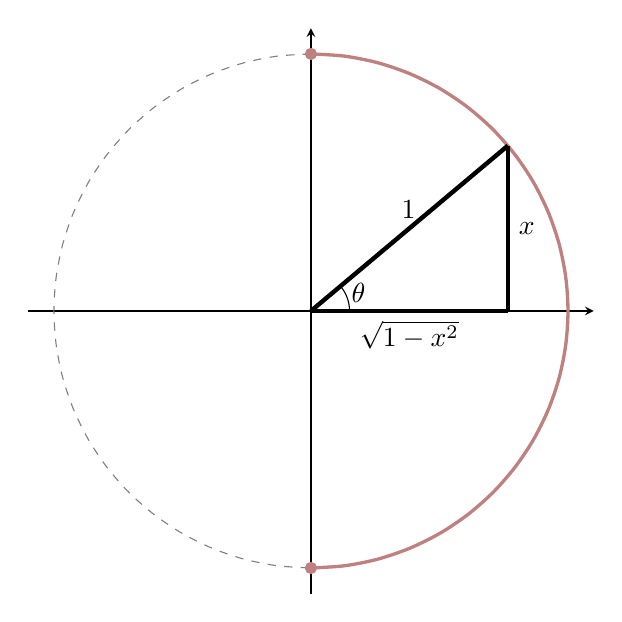
\begin{tikzpicture}
      \begin{axis}[
          xmin=-1.1,xmax=1.1,ymin=-1.1,ymax=1.1,
          axis lines=center,
          width=4in,
          ticks=none,
          clip=false,
          unit vector ratio*=1 1 1,
          %xlabel=$x$, ylabel=$y$,
          every axis y label/.style={at=(current axis.above origin),anchor=south},
          every axis x label/.style={at=(current axis.right of origin),anchor=west},
        ]        
        \addplot [penColor2!50!white, very thick, smooth, domain=(-90:90)] ({cos(x)},{sin(x)}); %% unit circle
        \addplot [black!50!white, dashed, smooth, domain=(90:270)] ({cos(x)},{sin(x)}); %% unit circle
        \addplot[color=penColor2!50!white,fill=penColor2!50!white,only marks,mark=*] coordinates{(0,1)};  %% closed hole
        \addplot[color=penColor2!50!white,fill=penColor2!50!white,only marks,mark=*] coordinates{(0,-1)};  %% closed hole         
        \addplot [ultra thick] plot coordinates {(0,0) (.766,.643)}; %% 40 degrees
        
        \addplot [ultra thick] plot coordinates {(.766,0) (.766,.643)}; %% 40 degrees
        \addplot [ultra thick] plot coordinates {(0,0) (.766,0)}; %% 40 degrees
        
        %\addplot [ultra thick,penColor3] plot coordinates {(1,0) (1,.839)}; %% 40 degrees          
        
        \addplot [textColor,smooth, domain=(0:40)] ({.15*cos(x)},{.15*sin(x)});
        %\addplot [very thick,penColor] plot coordinates {(0,0) (.766,.643)}; %% sector
        %\addplot [very thick,penColor] plot coordinates {(0,0) (1,0)}; %% sector
        %\addplot [very thick, penColor, smooth, domain=(0:40)] ({cos(x)},{sin(x)}); %% sector
        \node at (axis cs:.12,.07) [anchor=west] {$\theta$};
        \node at (axis cs:.84,.322) {$x$};
        \node at (axis cs:.383,0) [anchor=north] {$\sqrt{1-x^2}$};
        \node at (axis cs:.38,.32) [anchor=south] {$1$};
      \end{axis}
    \end{tikzpicture}
  \end{image}
  From the unit circle above, we see that 
  \begin{align*}
    \theta' &= \frac{1}{\cos(\theta)}\\
    &=\frac{\mathrm{hyp}}{\mathrm{adj}}\\
    &= \answer[given]{\frac{1}{\sqrt{1-x^2}}}.
  \end{align*}
   Recall, $\cos{x}\ge0$ on the interval $\Bigl(-\frac{\pi}{2},\frac{\pi}{2}\Bigr)$.\\
   
  To be completely explicit, 
  \[
  \ddx \theta = \ddx \arcsin(x) = \answer[given]{\frac{1}{\sqrt{1-x^2}}}.
  \]
 
\end{explanation}
\end{theorem}


\begin{question}
  Compute:
  \[
  \ddx \sin^{-1}(x)
  \begin{prompt}
    = \answer[given]{1/\sqrt{1-x^2}}
  \end{prompt}
  \]
\end{question}



We can do something similar with arctangent. 


\begin{theorem}[The derivative of arctangent]\index{derivative!of arctangent}
  \[
  \ddx \arctan(x) = \frac{1}{1+x^2}.
  \]
  \begin{explanation} 
     To start, note that the Inverse Function Theorem assures us that this
     derivative actually exists.
    Recall
    \[
    \arctan(x) = \theta
    \]
    means that $\tan(\theta) = x$ and $\answer[given]{\frac{-\pi}{2}}<
    \theta< \answer[given]{\frac{\pi}{2}}$.  Implicitly
    differentiating with respect $x$ we see
    \begin{align*}
      \tan(\theta) &= x\\
      \ddx \tan(\theta) &= \ddx x         &\text{Differentiate both sides.}\\
      \sec^2(\theta) \cdot \theta' &= 1   &\text{Implicit differentiation.}\\
      \theta' &= \frac{1}{\sec^2(\theta)} 
       \end{align*}
      Recall the trig identity:  $\sec^2(\theta)=1+\tan^2(\theta)$.\\
        \begin{align*}
          \theta' &= \frac{1}{1+\tan^2(\theta)} 
         \end{align*}
         Recall from above:  $\tan(\theta) = x$.\\
          \begin{align*}
          \theta' &= \frac{1}{1+x^2} 
         \end{align*}
  %%  While $\theta' = \cos^2(\theta)$, we need our answer written in terms
    %of $x$. Since we are assuming that
   % \[
   % \tan(\theta) = \frac{\sin(\theta)}{\cos(\theta)}= x,
   % \]
   % we may consider the following triangle:
    %\begin{image}[2in]
     % \begin{tikzpicture}
      %  \coordinate (A) at (5*.766,5*0);
        %\coordinate (B) at (5*.766,5*.643);
       % \coordinate (C) at (0,0);
       % \tkzMarkRightAngle(C,A,B)
        %\tkzMarkAngle[size=.6cm,thin](A,C,B)
        
	%\draw[very thick] (A)--(B)--(C)--cycle;
        %\node at (5*.10,5*.06) [anchor=west] {$\theta$};
       % \node at (5*.766,5*.322)[anchor=west] {$x$};
       % \node at (5*.383,0) [anchor=north] {$1$};
        %\node at (5*.38,5*.32) [above left] {$\sqrt{1+x^2}$};
   % \end{tikzpicture}
    %\end{image}
    %We may now scale this triangle by a factor of $\frac{1}{\sqrt{1+x^2}}$ to place
   % it on the unit circle:
   % \begin{image}
      %\begin{tikzpicture}
	%\begin{axis}[
           % xmin=-1.1,xmax=1.1,ymin=-1.1,ymax=1.1,
            %axis lines=center,
            %width=4in,
            %ticks=none,
           % clip=false,
           % unit vector ratio*=1 1 1,
            %xlabel=$x$, ylabel=$y$,
           % every axis y label/.style={at=(current axis.above origin),anchor=south},
           % every axis x label/.style={at=(current axis.right of origin),anchor=west},
        %  ]        
         % \addplot [penColor3!50!white, very thick, smooth, domain=(-90:90)] ({cos(x)},{sin(x)}); %% unit circle
          %\addplot [black!50!white, dashed, smooth, domain=(90:270)] ({cos(x)},{sin(x)}); %% unit circle
          %\addplot[color=penColor3!50!white,fill=white,only marks,mark=*] coordinates{(0,1)};  %% open hole
          %\addplot[color=penColor3!50!white,fill=white,only marks,mark=*] coordinates{(0,-1)};  %% open hole     
          %\addplot [ultra thick] plot coordinates {(0,0) (.766,.643)}; %% 40 degrees

         % \addplot [ultra thick] plot coordinates {(.766,0) (.766,.643)}; %% 40 degrees
         % \addplot [ultra thick] plot coordinates {(0,0) (.766,0)}; %% 40 degrees
          
          %\addplot [ultra thick,penColor3] plot coordinates {(1,0) (1,.839)}; %% 40 degrees          

         % \addplot [textColor,smooth, domain=(0:40)] ({.15*cos(x)},{.15*sin(x)});
          %\addplot [very thick,penColor] plot coordinates {(0,0) (.766,.643)}; %% sector
          %\addplot [very thick,penColor] plot coordinates {(0,0) (1,0)}; %% sector
          %\addplot [very thick, penColor, smooth, domain=(0:40)] ({cos(x)},{sin(x)}); %% sector
         % \node at (axis cs:.12,.07) [anchor=west] {$\theta$};
         % \node at (axis cs:.84,.322)[anchor=west] {$\frac{x}{\sqrt{1+x^2}}$};
         % \node at (axis cs:.383,0) [anchor=north] {$\frac{1}{\sqrt{1+x^2}}$};
          %\node at (axis cs:.38,.32) [anchor=south] {$1$};
        %\end{axis}
%\end{tikzpicture}
%\end{image}
%%From the unit circle above, we see that 
%%\begin{align*}
%%  \theta' &= \cos^2(\theta)\\
 %% &= \left(\frac{\mathrm{adj}}{\mathrm{hyp}}\right)^2\\
  %&= \answer[given]{\frac{1}{1+x^2}}.
%%\end{align*}
To be completely explicit, 
\[
\ddx \theta = \ddx \arctan(x) = \answer[given]{\frac{1}{1+x^2}}.
\]
\end{explanation}
\end{theorem}

\begin{question}
  Compute:
  \[
  \ddx \tan^{-1}(\sqrt{x})
  \begin{prompt}
    = \answer[given]{1/(2\sqrt{x}(1+x))}
  \end{prompt}
  \]
\end{question}



Finally, we investigate the derivative of arcsecant.

\begin{theorem}[The derivative of arcsecant]\index{derivative!of arcsecant}
\[
\ddx \arcsec(x) = \frac{1}{|x|\sqrt{x^2-1}}\qquad\text{for $|x|>1$.}
\]
\begin{explanation} 
  %% To start, note that the Inverse Function Theorem assures us that this
  %% derivative actually exists.
  Recall
\[
\arcsec(x) = \theta
\]
means that $\sec(\theta) = x$ and $\answer[given]{0}\le \theta\le
\answer[given]{\pi}$ with $\theta\ne \answer[given]{\pi/2}$.  Implicitly
differentiating with respect $x$ we see
\begin{align*}
\sec(\theta) &= x\\
\ddx \sec(\theta) &= \ddx x                     &\text{Differentiate both sides.}\\
\sec(\theta)\tan(\theta) \cdot \theta' &= 1     &\text{Implicit differentiation.}\\
\theta' &= \frac{1}{\sec(\theta)\tan(\theta)}   &\text{Solve for $\theta'$.}\\
\theta' &= \frac{\cos^2(\theta)}{\sin(\theta)}.
\end{align*}
While $\theta' = \frac{\cos^2(\theta)}{\sin(\theta)}$, we need our
answer written in terms of $x$. Since we are assuming that
\[
\sec(\theta) = \frac{1}{\cos(\theta)}= x,
\]
we may consider the following triangle:
    \begin{image}[2in]
      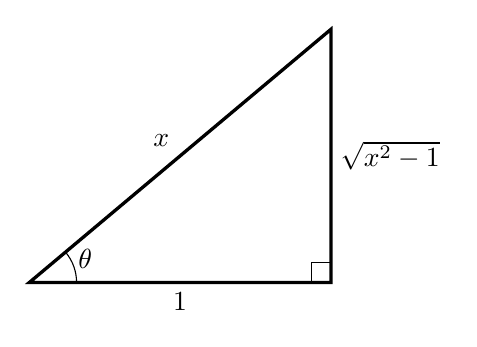
\begin{tikzpicture}
        \coordinate (A) at (5*.766,5*0);
        \coordinate (B) at (5*.766,5*.643);
        \coordinate (C) at (0,0);
        \tkzMarkRightAngle(C,A,B)
        \tkzMarkAngle[size=.6cm,thin](A,C,B)
        
	\draw[very thick] (A)--(B)--(C)--cycle;
        \node at (5*.10,5*.06) [anchor=west] {$\theta$};
        \node at (5*.766,5*.322)[anchor=west] {$\sqrt{x^2-1}$};
        \node at (5*.383,0) [anchor=north] {$1$};
        \node at (5*.38,5*.32) [above left] {$x$};
    \end{tikzpicture}
    \end{image}
    We may now scale this triangle by a factor of $\frac{1}{x}$ to place
    it on the unit circle:
\begin{image}
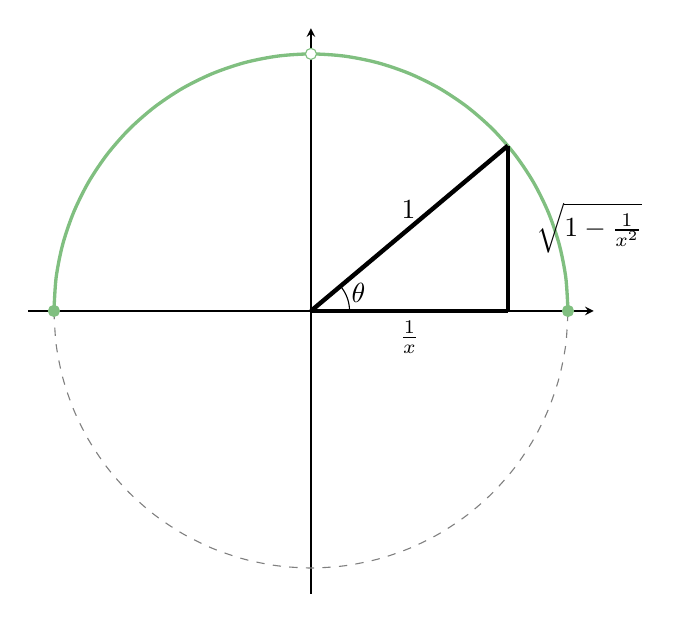
\begin{tikzpicture}
	\begin{axis}[
            xmin=-1.1,xmax=1.1,ymin=-1.1,ymax=1.1,
            axis lines=center,
            width=4in,
            ticks=none,
            clip=false,
            unit vector ratio*=1 1 1,
            %xlabel=$x$, ylabel=$y$,
            every axis y label/.style={at=(current axis.above origin),anchor=south},
            every axis x label/.style={at=(current axis.right of origin),anchor=west},
          ]        
          \addplot [penColor4!50!white, very thick, smooth, domain=(0:180)] ({cos(x)},{sin(x)}); %% unit circle
          \addplot [black!50!white, dashed, smooth, domain=(180:360)] ({cos(x)},{sin(x)}); %% unit circle
          \addplot[color=penColor4!50!white,fill=white,only marks,mark=*] coordinates{(0,1)};  %% open hole
          \addplot[color=penColor4!50!white,fill=penColor4!50!white,only marks,mark=*] coordinates{(1,0)};  %% closed hole
          \addplot[color=penColor4!50!white,fill=penColor4!50!white,only marks,mark=*] coordinates{(-1,0)};  %% closed hole     
          \addplot [ultra thick] plot coordinates {(0,0) (.766,.643)}; %% 40 degrees

          \addplot [ultra thick] plot coordinates {(.766,0) (.766,.643)}; %% 40 degrees
          \addplot [ultra thick] plot coordinates {(0,0) (.766,0)}; %% 40 degrees
          
          %\addplot [ultra thick,penColor3] plot coordinates {(1,0) (1,.839)}; %% 40 degrees          

          \addplot [textColor,smooth, domain=(0:40)] ({.15*cos(x)},{.15*sin(x)});
          %\addplot [very thick,penColor] plot coordinates {(0,0) (.766,.643)}; %% sector
          %\addplot [very thick,penColor] plot coordinates {(0,0) (1,0)}; %% sector
          %\addplot [very thick, penColor, smooth, domain=(0:40)] ({cos(x)},{sin(x)}); %% sector
          \node at (axis cs:.12,.07) [anchor=west] {$\theta$};
          \node at (axis cs:.84,.322)[anchor=west] {$\sqrt{1-\frac{1}{x^2}}$};
          \node at (axis cs:.383,0) [anchor=north] {$\frac{1}{x}$};
          \node at (axis cs:.38,.32) [anchor=south] {$1$};
        \end{axis}
\end{tikzpicture}
\end{image}
From the unit circle above, we see that 
\begin{align*}
  \theta' &= \frac{\cos^2(\theta)}{\sin(\theta)}\\
  &= \frac{
    \left(\frac{\mathrm{adj}}{\mathrm{hyp}}\right)^2}{\frac{\mathrm{opp}}{\mathrm{hyp}}}\\
  &= \frac{\left(\mathrm{adj}\right)^2}{\mathrm{opp}} &\text{Note, $\mathrm{hyp}=1$.}\\
  &= \frac{\answer[given]{1/x^2}}{\sqrt{1-1/x^2}}\\
  &= \frac{1}{|x|\sqrt{x^2-1}},
\end{align*}
To be completely explicit, 
\[
\ddx \theta = \ddx \arcsec(x) = \frac{1}{|x|\sqrt{x^2-1}}\qquad\text{for $|x|>1$}. 
\]
\end{explanation}
\end{theorem}

\begin{question}
  Compute:
  \[
  \ddx \sec^{-1}(3x)
  \begin{prompt}
    = \answer[given]{\frac{1}{|x|\sqrt{(3x)^2-1}}}
  \end{prompt}
  \]
\end{question}

We leave it to you, the reader, to investigate the derivatives of
cosine, arccosecant, and arccotangent. However, as a gesture of
friendship, we now present you with a list of derivative formulas for
inverse trigonometric functions.

\begin{theorem}[The Derivatives of Inverse Trigonometric Functions] \hfil
\begin{itemize}
\item $\dd{x} \arcsin(x) = \frac{1}{\sqrt{1-x^2}}$
\item $\dd{x} \arccos(x) = \frac{-1}{\sqrt{1-x^2}}$
\item $\dd{x} \arctan(x) = \frac{1}{1+x^2}$
\item $\dd{x} \arcsec(x) = \frac{1}{|x|\sqrt{x^2-1}}$ for $|x|>1$
\item $\dd{x} \arccsc(x) = \frac{-1}{|x|\sqrt{x^2-1}}$ for $|x|>1$
\item $\dd{x} \arccot(x) = \frac{-1}{1+x^2}$
\end{itemize}
\end{theorem}








\end{document}
